\chapter{Act I}



\begin{figure}
    \centering
    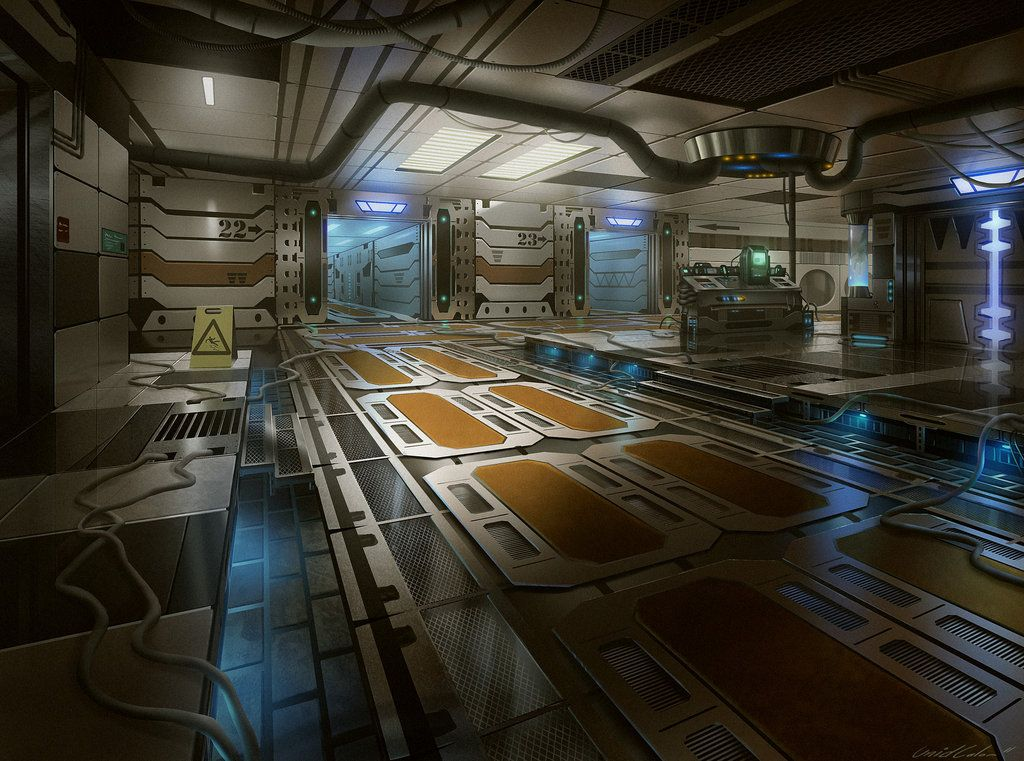
\includegraphics[width=.45\textwidth]{img/bg/interior.jpg}
\end{figure}



\begin{rpg-commentbox}{Chilling out}

    It is another day in the fire station. Paramedics are just tired of attending shift workers that overdose on never-sleeping pills. Firefighters are enjoying their meal and talking about whatever amenities they must talk about.

    \texttt{\textbf{MU/TH/UR:}} Let PCs have some time talking among themselves, play some rivalries and use NPC firefighters to guide the conversation if need be.
\end{rpg-commentbox}

\newsect

\begin{rpg-commentbox}{Fire alert}
    It would be yet another boring day for the majority of the crew when APOLLO puts the station on lock-down. There has been a huge fire and all non-essential personnel must remain on their quarters. Firefighters should proceed to San Cristobal Medical Facility immediately. 
    Traveling uses the Anchorpoint transit system. Each major section of the station has a firetruck and once out of rapid transit, firefighters can drive the truck through the station corridors. 

    \texttt{\textbf{MU/TH/UR:}} Use this time to roleplay the station chief. Debrief the situation, and what are the firefighters' priorities.
\end{rpg-commentbox}


\begin{rpg-commentbox}{Priorities}
    \begin{enumerate}
        \item Clear a path to the ambulance bay. Close hatches to suck all air of the bay, which is the primary source for the engulfing fire;
        \item Clear a path to the room (unknown designation) in between the staff quarters and environment control room. Secure any survivors in the room.
        \item Clear a path to the staff quarters where magnetic tapes and floppy data is kept. Save as much of the data as you can.
    \end{enumerate}
\end{rpg-commentbox}



\begin{rpg-commentbox}{Splitting the party}
    \texttt{\textbf{MU/TH/UR:}} Firefighters are in borrowed time. It's likely that they will have to split to cover all main objectives. Encourage that to the players and state that this is normal procedure. 

    It's not an alien game if everyone stays together watching each others back, right?
\end{rpg-commentbox}  

\begin{rpg-commentbox}{}
    \textbf{Act 1 ends when firefighters meet the Alien OR complete 2/3 of the objectives}
 \end{rpg-commentbox}

 \newsect


\section{Special Rules}

\begin{rpg-commentbox}{Air supply}
    Players start with air tanks at full capacity (\texttt{\textbf{AIR 5}}). Roll for air whenever firefighters move into a new zone (other than the first). Roll for air after major checks, for example when a player rolls for \texttt{\textbf{HEAVY MACHINERY}} to open a hatch that is stuck or \texttt{\textbf{COMM TECH}} to override a control panel.

    Firefighters often carry an extra air tank if they know that the situation requires it. 
    There may be occasional supplies in strategic locations at the facility. It's up to the game \texttt{\textbf{MU/TH/UR}} to decide if players suffocate [for a bit] or if they can find them, but word of advice is that this will always keep players in their toes. 
\end{rpg-commentbox}  


\begin{rpg-commentbox}{Stress}
    When in duty, firefighters do not take any \texttt{\textbf{STRESS}} for eventual victims that they find. This may come as an aftershock.

    Firefighters often carry \texttt{\textbf{NAPROLEVE}} with them. They use the medicine to reduce their stress before it gets too critical, but due to regulations, a maximum of one dose is available to each player if the game \texttt{\textbf{MU/TH/UR}} decides so. Strongly recommended as this scenario barely has any places/moments where a player can reduce stress. 
\end{rpg-commentbox}   





\section{Ambulance Bay}

\begin{rpg-commentbox}{The area}
    The ambulance bay is a small hangar with double-pressurized doors that allows landing of small shuttles. 
    It directly connects to the crisis stabilization center where any ICU patients are located. In the crisis stabilization area, there are 4 auto doc units and 2 auxiliary rooms for staff. A third 
    cylindrical room holds equipments and a small thermal battery can keep the area running even under the most dire situations.
    
    \texttt{\textbf{MU/TH/UR:}} One would have imagined that the patient brought by Weyland-Yutani would be here, but they are nowhere to be found.
\end{rpg-commentbox}  




\begin{rpg-commentbox}{Clearing a path}
    When firefighters get into the stabilization zone unit, the close the hatch behind them. There are three zones that they must  move through, each one representing one corridor after the initial corridor that marks the entrance.
    
    Due to the diamond shape format of the area, this 3 zones path is the same regardless if firefighters decide to take the right corridor or the left one.
    
    \texttt{\textbf{MU/TH/UR:}} Important details per zone/corridor:
    
    \texttt{\textbf{1st}} A firefighter that succeeds in a \texttt{\textbf{MOBILITY}} roll can safely reach the second corridor. Failure makes them fall, taking 1 point of damage, but still making the trip.

    \texttt{\textbf{2nd}} Once in 2nd corridor, a firefighter can cordinate with one that stayed at the entrance to use their tools to roll \texttt{\textbf{HEAVY MACHINERY}} (+2 if using a  \texttt{\textbf{halligan}}) to seal the 1st corridor and vent it, extinguishing any fire in the area. 

    While there is not as much fire here, visibility in this corridor is minimum and firefighters need to crouch and find their way to the next corridor. 
    \texttt{\textbf{MOBILITY}}, \texttt{\textbf{SURVIVAL}}, or \texttt{\textbf{SURVIVAL}} are options. Failure implies that a firefighter enters one of the ICU rooms losing precious time and forcing a roll on their air supply before they get to the final 3rd corridor.  

    \texttt{\textbf{3rd}} Once again, a \texttt{\textbf{HEAVY MACHINERY}} roll will make the previous corridor safe for passage for any other firefighters. When venting the second corridor, a patient that was in the floor suffocates. If you are comfortable, narrate their peril (see suffocating box).
    
    The fire here is extreme. The best option is to find hatches/panel of the fire supression system and try to manually trigger it filling the room with halon. 
    A \texttt{\textbf{COMM TECH}} roll can trigger the suppression mechanism.
    Contact of halon with some of the medical equipment in the area releases 
    noxious elements in the air. 
\end{rpg-commentbox}  


\begin{rpg-warnbox}{Suffocating}
    When the air is being venting out from the room a patient that was trapped starts to crawl towards one of the hatches. Firefighters see everything through the glass window. The patient grasps for air as the corridor eventually reaches zero-g and the body that was trapped calmly floats. Once the hatches are open, the body falls down and firefighters are reminded that ``\textit{in space no one can hear you screen}''.
\end{rpg-warnbox}
  

\newsect


\begin{rpg-commentbox}{Ambulance bay}
    Most of the structure is compromised here. Firefighters need to reach the hangar doors panel and initiate the standard landing procedures what will open the shuttle door and eventually leave the bay in vacuum. 

    The panel is too damaged for a \texttt{\textbf{COMM TECH}}, so firefighters need to do it manually. Pumping the lever does require  physical effort and the lever needs to be pushed thrice before it starts the standard landing procedures. 

    \texttt{\textbf{MU/TH/UR:}} Players can rotate who pushes the pump, but anyone who does it must immediately roll for \texttt{\textbf{AIR}}. If a single player does it, that means 3 consecutive rolls.
\end{rpg-commentbox}  

\newsect


\begin{rpg-commentbox}{Conclusion}
    Only smoke remains in the area, but most of the fire has been dealt with. Multiple bodies can be found through the corridors, but they are the expected casualties.
    
    \texttt{\textbf{MU/TH/UR:}} The fire chief communicates with the firefighters in the area commending them for their job  and ordering them to proceed either to the mysterious room zone or the data drive area. 

    The chief's appraisal reassures the firefighters, relieve \texttt{\textbf{1 STRESS}} from any players who were in the area.
\end{rpg-commentbox}  



\clearpage

\section{Mysterious Room}



\begin{figure}
    \centering
    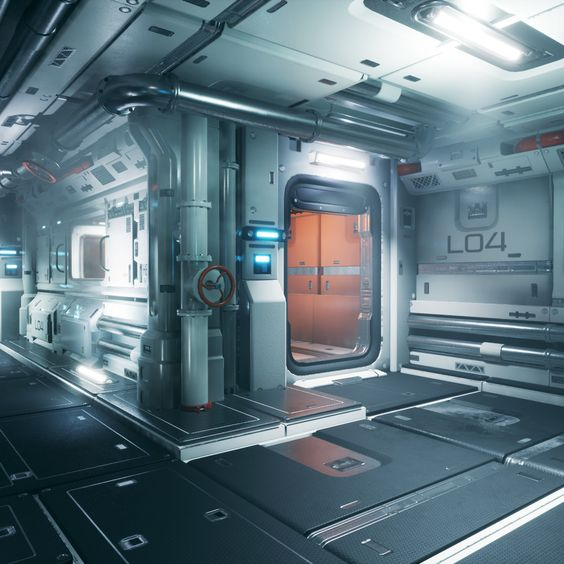
\includegraphics[width=.4\textwidth]{img/bg/corridor.jpg}
\end{figure}


\begin{rpg-commentbox}{The area}
    This room is located close to the sedation ward and near the entrance of the staff quarters where data drivers are located. It is bigger than any ICU in the crisis stabilization center and it is in fact the most well equipped ICU in the facility.

    It's purpose is to house any VIP with medical issues in a secure location away from any curious eyes. The \texttt{\textbf{VIP ICU}} also has equipment for biopsies and containment of any foreign substance or parasite that might be found. 

    This is particularly important in case of viruses, as companies, such as Lasalle Bionational, are always in the look for new chemical compounds or elements that can be bio-engineered and turned into assets.

    The fire has not spread to this area yet. The two nearby areas, environment control and the sedation ward have fires. A skilled firefighter will notice that fire in these areas is not expected if the source of fire is in the ambulance bay.

    \texttt{\textbf{MU/TH/UR:}} One unfortunate person lies dead in an auto doc pod.
    It's clearly visible that they were restrained and their stomach is open. Even the firefighters take a \texttt{\textbf{STRESS}} point.

    There is liquid dripping from one of the biopsy pods that is shattered. Further inspection shows one medic or scientist dead. After the appropriate check a firefighter can uncover that the medic had their ankle cut open and thus, they bleed to death. 
\end{rpg-commentbox}   



\begin{rpg-commentbox}{Clearing a path}
    The shortest path from the entrance to the mysterious room is through the assessment area. Patients are checked here and in case of grave injuries led to the crisis stabilization area. Otherwise, patients proceed to the sedation ward area where minor injuries are treated and antibiotics administered. 
    
    There are again three zones until the mysterious room front door. They are the assessment room itself, an auxiliary area that leads to the environmental control room and  that also has a set of stairs to other areas of the facility and finally, a connecting corridor that leads to the mysterious room.
    
    \texttt{\textbf{MU/TH/UR:}} Important details per zone in the following boxes.
\end{rpg-commentbox}      

\begin{rpg-commentbox}{Clearing a path - Assessment Room}
    The hatch to this room was automatically closed by APOLLO---unknown if due to a malfunction or due to standard procedures. As the firefighters open the hatch, a cloud of smoke erupts making visibility hard. Even worse, several patients and staff who were in the room storm the firefighters asking for help and trying to grab any of their equipment in hopes of finding a respiration mask. 

    A \texttt{\textbf{COMMAND}} roll can calm down the distressed victims and they can crouch to the exit themselves. A \texttt{\textbf{CLOSE COMBAT}} can be also used to to escape from the mob. 
    Failure means a \texttt{\textbf{STRESS}} point and a roll for \texttt{\textbf{AIR}}.

    Most people here are visibly shaken and some of them ask if the firefighters ``\textit{have seen it}''. If asked about what the victims mumble and do not say anything coherent. 
\end{rpg-commentbox}  



\begin{rpg-commentbox}{Clearing a path - Auxiliary Room}
    Firefighters notice a raging fire coming from the sedation ward zone. The smoke from the fire area once again difficulties vision. 
    It's strange because the source of the fire should be the ambulance bay. To the south there is the environmental control room and stairs leading to the objective. 
    
    If firefighters decide to stop and check environmental control, they can try to manually override stuck halon ``sprinklers' and perhaps suppress the fire in other areas of the facility. 
    A \texttt{\textbf{OBSERVATION}} roll shows that the pipes/tubes leading to the sedation ward have been damaged but auxiliary canisters should have been fired.
    \texttt{\textbf{COMM TECH}} allows a firefighter to hack environmental control and activate the fire suppressing mechanism. 
    Stopping at environmental control means a roll for \texttt{\textbf{AIR}}.


    When moving from the stair set, part of the celling and ventilation collapses. 
    Roll for \texttt{\textbf{MOBILITY}} to dodge. Failure means rolling 
    \texttt{\textbf{5 DAMAGE}}.
    
    While there is not as much fire here, visibility in this corridor is minimum and firefighters need to crouch and find their way to the next corridor. 
    \texttt{\textbf{MOBILITY}}, \texttt{\textbf{SURVIVAL}}, or \texttt{\textbf{SURVIVAL}} are options. Failure implies that a firefighter enters one of the ICU rooms losing precious time and forcing a roll on their air supply before they get to the final 3rd corridor.  
\end{rpg-commentbox}  



\clearpage

\begin{rpg-commentbox}{Clearing a path - Connecting Corridor}    
    After the structural damage, the door at the end of the corridor is stuck.
    \texttt{\textbf{HEAVY MACHINERY}} can pry it open. 
    A roll with a \texttt{\textbf{halligan}} is made at -2 while a hydraulic rescue tool such as a \texttt{\textbf{spreader}} allows a straight check.

    Failure here is a major setback because it means that the path is blocked and firefighters must go through the crisis stabilization path to get to the mysterious room. 
\end{rpg-commentbox}  



\begin{rpg-commentbox}{Conclusion}
    With no VIP patient in sight, only the data drivers can explain what happened in this room.
    
    \texttt{\textbf{MU/TH/UR:}} The fire chief communicates with the firefighters in the area commenting that these events are really unsettling and that he has never heard or seen anything similar. He will reach out to Weyland-Yutani operatives and see if they are hiding anything. He order the firefighters to fetch the drivers in the server room.
\end{rpg-commentbox}  

\makebox[0pt][l]{%
  \raisebox{-\totalheight}[120pt][0pt]{%
    \hspace*{-0.5cm}%
    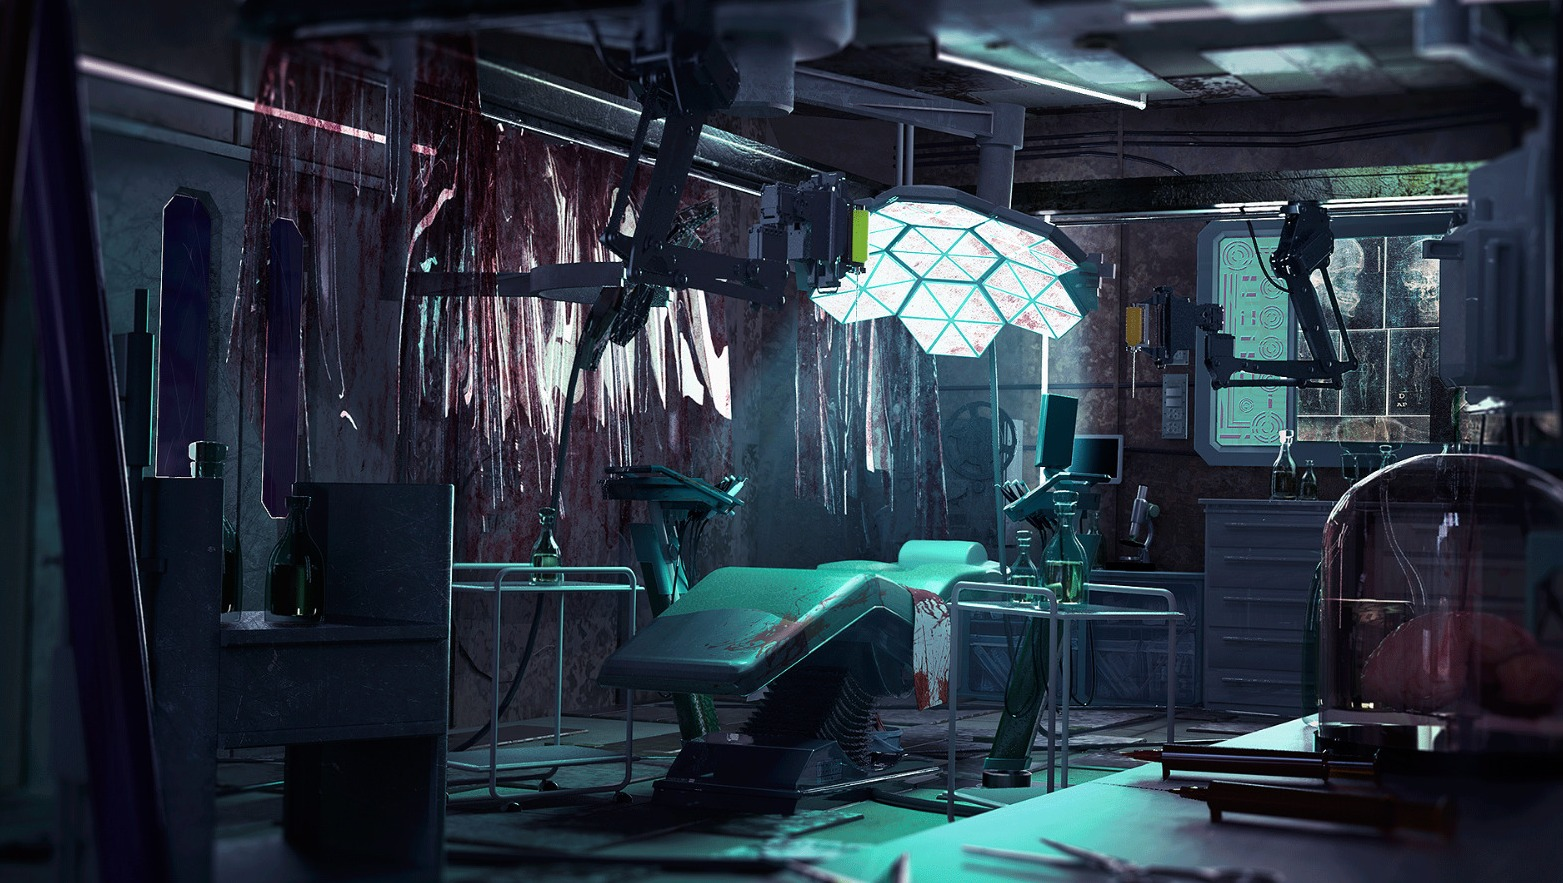
\includegraphics[width=1.0\textwidth]{img/bg/lab-2.jpeg}}}%

% \begin{figure*}
%     \centering
%     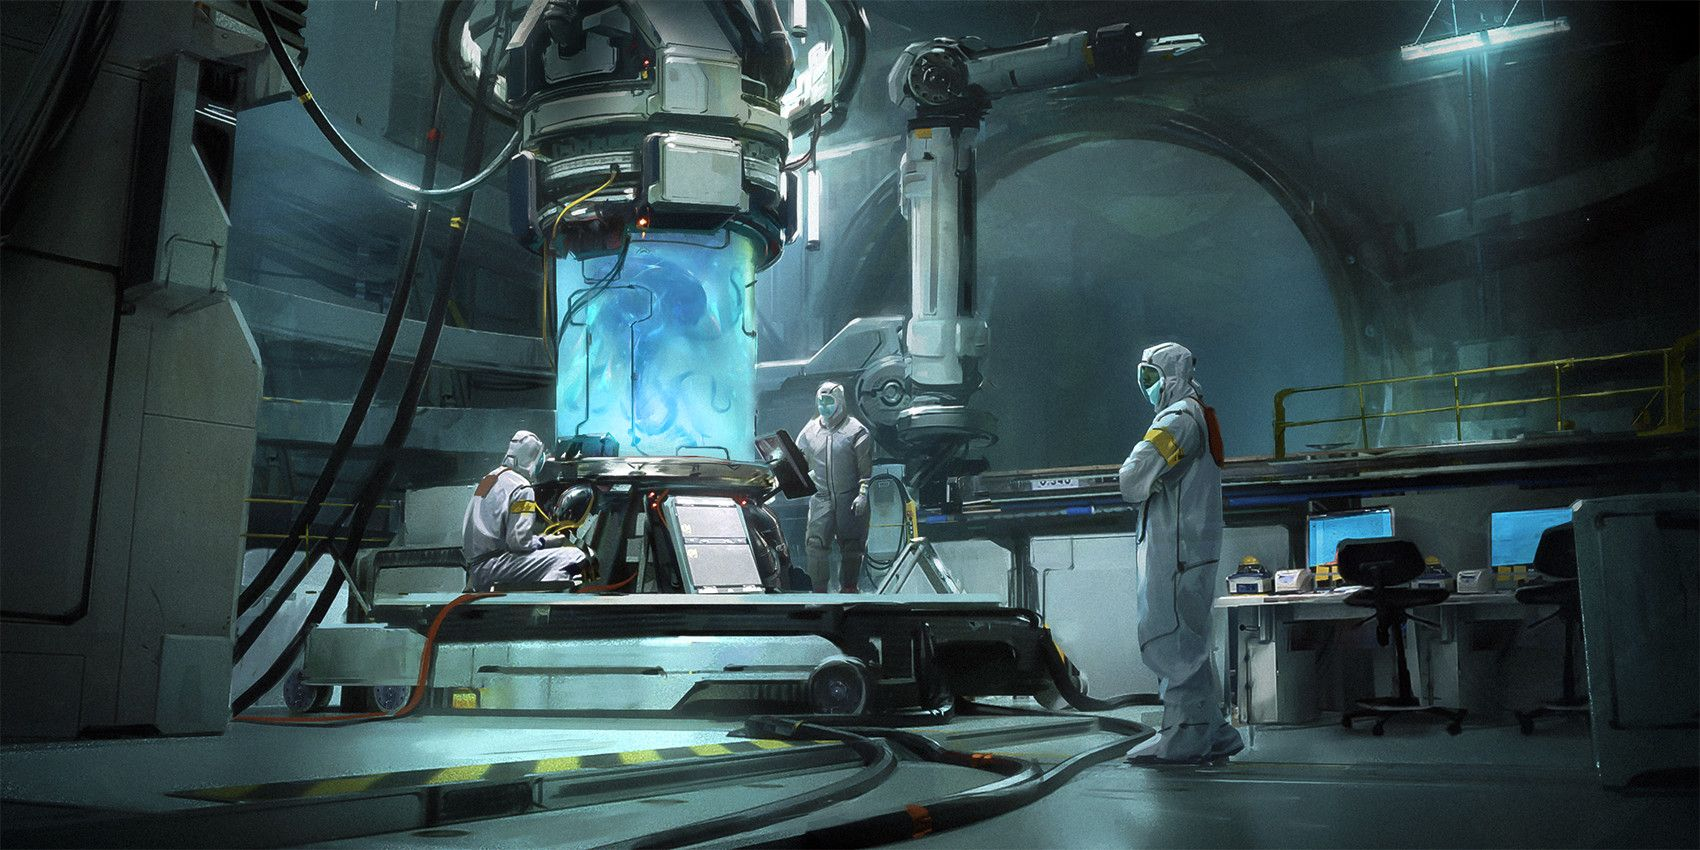
\includegraphics[width=.95\textwidth]{img/bg/lab.jpg}
% \end{figure*}

\clearpage

\section{Data Drivers}


\begin{figure}
    \centering
    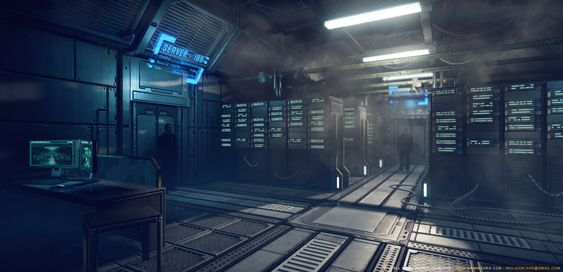
\includegraphics[width=.45\textwidth]{img/bg/server.jpg}
\end{figure}


\begin{rpg-commentbox}{The area}
    This area is where the facility personnel rest and relax whenever they are not in a shift. There is a kitchen, cabinets, chemical showers, and bunk beds in the area. 
    
    The far north-east corner of the area also has the computational grid and data drivers of the facility. One would expect a dedicated room or area for that but it seems that the staff quarters were actually pushed to the server room as the facility grew in size. 

    A few staff members are in the area, including a comm expert that is frenetically going over the data grids as two Weyland-Yutani mercenaries watch him. 

    \texttt{\textbf{MU/TH/UR:}} The entrance door is barred. \texttt{\textbf{HEAVY MACHINERY}} or \texttt{\textbf{COMM TECH}} can force it open. As soon as the door is about to open, jump to end of act 1.
\end{rpg-commentbox}  


\begin{rpg-commentbox}{Clearing a path}
    If the firefighters made their way to the mysterious room, the staff quarters should already be accessible. 

    If the firefighters made their way though the crisis stabilization area, they must pass through two other zones to get to the staff quarters: a long corridor that connects the unit to the facility power plant and warehouse and the plant/warehouse itself. 
    
    \texttt{\textbf{MU/TH/UR:}} Important details per zone in the following boxes.
\end{rpg-commentbox}



\begin{rpg-commentbox}{Clearing a path - Warehouse corridor}
    As soon as the firefighters open the hatch to the corridor, air starts to escape the room. It seems that the clash has cause a rupture in the corridor windows which provided a scenic view to space. Firefighters must use their ropes and grappling hooks to reach the emergency lever that will seal the windows with a heavy metal panels that are retracted on the corridor celling.
    
    A \texttt{\textbf{MOBILITY}} roll allows a firefighter to reach the panels. Failure implies losing their grip and flying towards the whole in the window. Roll \texttt{\textbf{4 DAMAGE}} for the impact of flying while debris in the room is also being sucked. 
\end{rpg-commentbox}




\begin{rpg-commentbox}{Clearing a path - Warehouse}
    This decommissioned section is serving as a temporary warehouse. To the south lies the facility power plant and further east, staff's offices (mostly HR and insurance).
    
    This area is strangely quiet amidst the chaos of the other zones. The only pressing problem is time, but firefighters can search the warehouse and perhaps find supplies. The pharmacy room is locked for security reasons, but a \texttt{\textbf{HEAVY MACHINERY}} or \texttt{\textbf{COMM TECH}} at -2 penalty can eventually open the door to the pharmacy.

    
    \texttt{\textbf{MU/TH/UR:}} If the firefighters take too much time looking for supplies, roll for \texttt{\textbf{AIR}}.

    
    
    \texttt{\textbf{Supplies:}} air canisters, first aid kits, alcohol, disinfectants, naproleve, and some other items that you deem important might be found through the warehouse and pharmacy.
\end{rpg-commentbox}

\newsect

\section{End of Act}




\begin{rpg-commentbox}{If you end once 2 objectives are completed:}
    \texttt{\textbf{MU/TH/UR:}} Narrate that other NPC firefighters that are in other areas of the facility open the firefighters common comm channel. 

    ``\textit{Chief! There is something else here! It impaled [NPC name]. Oh my god! Oh my god! It's comming for me chief, get us out of here, open the door.}''

    Anyone in the channel hears the sound of someone banging a metal door and an alien sound getting closer and closer. A huge final scream is heard. After that, the chief keeps calling for [NPC name].
\end{rpg-commentbox}



\begin{rpg-commentbox}{If you end once door to staff quarters opens:}
    \texttt{\textbf{MU/TH/UR:}} Narrate:

    When the door is about to be open one of the Weyland-Yutani mercenaries pull his sidearm pistol and makes a shhh sign with his finger. He starts to walk with his back against a wall while the other does the same in the opposite direction.
    
    ``\textit{The technical staff operating a computer screams as you see this huge black being fall behind the person. It puts its two hands on each site of the person's helmet and crashes it. The mercenaries panic and start shooting. One of the bullets hits a container that explodes and the magnetic tapes in the room quickly start a fire. Startled by the fire, the creature jumps back into the ventilation and the firefighters hear the thunk sound of its claws against the air ducts as it moves away.}''
\end{rpg-commentbox}